\documentclass[12pt,a4paper]{article}
\usepackage[utf8]{inputenc}
\usepackage[margin=2cm]{geometry}
\usepackage{amsmath}
\usepackage{amssymb}
\usepackage{amsthm} 
\usepackage{graphicx}
\usepackage{mathtools}
\usepackage{cancel}
\usepackage[normalem]{ulem}
\DeclarePairedDelimiter{\abs}{\lvert}{\rvert}
\newcommand{\inter}{\begin{matrix}\prod\end{matrix}}
\DeclarePairedDelimiter{\norma}{\lVert}{\rVert}
 
\begin{document}
\section{Lezione 20 - Condizionamento di matrici e sistemi lineari}

Grazie allo strumento delle norme vettoriali e matriciali indotte introdotto nella scorsa lezione, possiamo ``misurare" gli errori su vettori e matrici.\\
In questa lezione, utilizzando le due diseguaglianza fondamentali per le norme matriciali indotte
\begin{itemize}
    \item[(i)]$\norma{Ax} \leq \norma{A}\cdot\norma{x}$ (1$^\circ$ diseguaglianza fondamentale)
    \item[(ii)] $\norma{AB} \leq \norma{A} \cdot\norma{B}$ (2$^\circ$ diseguaglianza fondamentale)
\end{itemize}
vedremo come sia possibile stimare la ``risposta" di un sistema lineare non singolare agli errori sui dati
\begin{equation*}
    Ax=b, \ A\in \mathbb{R}^{n\times n}, \ b,x\in \mathbb{R}^n, \ det(A) \neq 0
\end{equation*}

\subsection{Perturbazioni in un sistema lineare}
Nelle applicazioni infatti sia la matrice $A$ che il vettore termine noto $b$ possono essere (e di solito sono) affetti da errori (in ogni caso gli arrotondamenti nel sistema floating-point, errori di misura sperimentale che sono di solito molto più grandi degli errori di arrotondamento, \dots).\\
Quindi in pratica ci si trova a risolvere un sistema ``perturbato"
\begin{equation*}
    \Tilde{A}\Tilde{x}=\Tilde{b}
\end{equation*}
dove $\Tilde{b}=b+\delta b$, $\Tilde{A}=A+\delta A$ cioè
\begin{equation*}
    \Tilde{b}= 
    \begin{pmatrix}
    \Tilde{b}_1\\  
    \vdots\\ 
    \Tilde{b}_n
\end{pmatrix} =
\begin{pmatrix}
    b_1\\  
    \vdots\\ 
    b_n
\end{pmatrix} + 
\begin{pmatrix}
    \delta b_1\\  
    \vdots\\ 
    \delta b_n
\end{pmatrix}
\end{equation*}
\begin{equation*}
    \Tilde{A} =
    \begin{pmatrix}
        \Tilde{a}_{11} & \dots & \Tilde{a}_{1n} \\
        \vdots & & \vdots \\
        \Tilde{a}_{n1} & \dots & \Tilde{a}_{nn}
    \end{pmatrix} = 
    \begin{pmatrix}
        a_{11} & \dots & a_{1n} \\
        \vdots & & \vdots  \\
        a_{n1} & \dots & a_{nn}
    \end{pmatrix} +
    \begin{pmatrix}
        \delta a_{11} & \dots & \delta a_{1n} \\
        \vdots & & \vdots \\
        \delta a_{n1} & \dots & \delta a_{nn}
    \end{pmatrix}
\end{equation*}
sono il vettore termine noto ``perturbato" e la matrice ``perturbata" a cui corrisponde un vettore soluzione ``perturbato" $\Tilde{x}=x+\delta x$
\begin{equation*}
    \Tilde{x}= 
    \begin{pmatrix}
    \Tilde{x}_1\\  
    \vdots\\ 
    \Tilde{x}_n
\end{pmatrix} =
\begin{pmatrix}
    x_1\\  
    \vdots\\ 
    x_n
\end{pmatrix} + 
\begin{pmatrix}
    \delta x_1\\  
    \vdots\\ 
    \delta x_n
\end{pmatrix}
\end{equation*}
Il problema di stimare $\delta x$ in funzione di $\delta b$ e $\delta A$ è detto problema di ``condizionamento" del sistema lineare corrispondente ad un'analisi di stabilità ``a monte" (stabilità del problema), prima di applicare algoritmi di calcolo della soluzione.
Cominciamo da una stima di base

\subsection{PROPOSIZIONE 1 (errore sulla soluzione di una sistema lineare generato da una perturbazione del termine noto)}
Sia $A \in \mathbb{R}^{n\times n}$ una matrice non singolare, $x \in \mathbb{R}^n$ soluzione del sistema $Ax=b$, $b \neq 0$ e $\Tilde{x}=x+\delta x$ soluzione del sistema perturbato $A\Tilde{x}=\Tilde{b}=b+\delta b$.\\
Fissata una norma vettoriale $\norma{\cdot}$ in $\mathbb{R}^n$, vale la seguente stima dell'errore ``relativo" su $x$
\begin{equation*}
    \frac{\norma{\delta x}}{\norma{x}} \leq k(A) \frac{\norma{\delta b}}{\norma{b}}
\end{equation*}
dove 
\begin{equation*}
    k(A)=\norma{A}\cdot\norma{A^{-1}}
\end{equation*}
prodotto della norma indotta di $A$ e $A^{-1}$, è detto ``INDICE (o anche numero) DI CONDIZIONAMENTO" della matrice $A$ (nella norma indotta).\\
\begin{proof}[\unskip\nopunct]
\textbf{Dimostrazione}\\Osserviamo che $x=A^{-1}b\neq0$ quindi ha senso stimare l'errore relativo in norma (cioè l'errore assoluto $\norma{\delta x}$ diviso per la ``lunghezza" di $x$, cioè $\norma{x}$). \\Ora
\begin{equation*}
    \tilde{x}=\cancel{x}+\delta x =A^{-1}\tilde{b}=A^{-1}(b+\delta b)=\cancel{A^{-1}}b+A^{-1}\delta b
\end{equation*}
da cui otteniamo la stima dell'errore assoluto
\begin{equation*}
    \norma{\delta x}=\norma{A^{-1}\delta b}\underset{1^o dis. fond.}{\leq}\norma{A^{-1}}\cdot\norma{\delta b}
\end{equation*}
Per stimare l'errore relativo dobbiamo stimare da sopra $\frac{1}{\norma{x}}$, cioè da sotto $\norma{x}$.\\Siccome $x$ è la soluzione 
\begin{equation*}
    \norma{b}=\norma{Ax}\underset{1^o dis. fond.}{\leq}\norma{A}\cdot\norma{x}
\end{equation*}
da cui
\begin{equation*}
    \norma{x}\geq\frac{\norma{b}}{\norma{A}}
\end{equation*}
e
\begin{equation*}
    \frac{1}{\norma{x}} \le \frac{\norma{A}}{\norma{b}}
\end{equation*}
perciò
\begin{equation*}
    \frac{\norma{\delta x}}{\norma{x}}\leq \frac{\norma{A^{-1}}\cdot\norma{\delta b}}{\norma{x}}\leq \norma{A^{-1}}\cdot\norma{A}\cdot\frac{\norma{\delta b}}{\norma{b}}=k(A)\cdot\frac{\norma{\delta b}}{\norma{b}}
\end{equation*}
\end{proof}
Facciamo subito alcune osservazioni:

\subsubsection{Proprietà 1}
$k(A)\geq1$ : infatti
\begin{equation*}
    k(A)=\norma{A^{-1}}\cdot\norma{A}\underset{1^o dis. fond.}{\geq}\norma{A^{-1}A}=\norma{I}=1
\end{equation*}
Quindi $k(A)$ nella stima ha il ruolo di ``amplificatore" dell'errore sui dati.\\ In molte applicazioni accade che $k(A) \gg 1$ : in questi casi si dice che il sistema è \uline{MAL CONDIZIONATO}, il che significa che piccole perturbazioni sui dati possono portare ad errori molto grandi sulla soluzione.\\
Non sono infrequenti sistemi di interesse in modelli applicativi per cui $k(A)\approx10^{20}$, $10^{30}$.\\In questi casi il sistema è ``estremamente" mal condizionato ed amplifica in modo tale perfino gli errori di arrotondamento delle componenti di $b$, che la soluzione può perdere completamente di significato perchè
\begin{equation*}
    \frac{\norma{\delta x}}{\norma{x}}>1
\end{equation*}
(cioè l'errore diventa maggiore del 100\%).\\Per queste situazioni estreme (e comunque quando $k(A)\cdot\frac{\norma{\delta b}}{\norma{b}}>1$) non ha molto senso calcolare la soluzione del sistema con algoritmi classici (che porterebbero alla soluzione perturbata con un errore inaccettabile) ma vanno costruiti metodi particolari che ``limitano" la perdita di precisione (come analogia, si pensi alla minimizzazione dell'errore in un altro classico problema molto instabile, quello del calcolo della derivata di una funzione perturbata; faremo un cenno facoltativo a questo tipo di approccio alla fine della lezione).\\Quando invece la situazione non è così estrema e $k(A)\cdot\frac{\norma{\delta b}}{\norma{b}}$ è ancora abbastanza piccolo, è comunque importante stimare $k(A)$ in qualche norma per avere un'idea di quanta precisione ci si aspetta di poter perdere rispetto alla precisione con cui sono noti i dati.\\In effetti $k(A)$ dipende dalla norma indotta che si usa: ad esempio chiameremo $k_\infty(A)$ l'indice di condizionamento rispetto alla $norma-\infty$, $k_2(A)$ quello rispetto alla $norma-2$ (indotte dalla corrispondenti norme vettoriali).\\In Matlab (come in tutti gli ambienti evoluti di calcolo) esistono funzioni predefinite per stimare l'ordine di grandezza dell'indice di condizionamento, ad es. in Matlab $cond(A) \approx K_2(A) = \norma{A}_2 \norma{A^{-1}}_2$ e $cond(A,Inf) \approx K_\infty(A) = \norma{A}_\infty \norma{A^{-1}}_\infty$.\\
Vale la pena di fare subito un semplice esempio, per fissare le idee.

\subsubsection*{Esempio}
Consideriamo il sistema $2\times 2$
\begin{equation*}
    \begin{cases}
        7x_1 + 10x_2 = b_1\\ 
        5x_1 + 7x_2 = b_2
    \end{cases}
\end{equation*}
con matrice (e inversa)
\begin{equation*}
    A=\begin{pmatrix}
        7 & 10 \\
        5 & 7
    \end{pmatrix}, \
    A^{-1}=\begin{pmatrix}
        -7 & 10 \\
        5 & -7 
    \end{pmatrix}
\end{equation*}
Prendiamo 
    $b=\bigl(\begin{smallmatrix}
    b_1 \\
    b_2
\end{smallmatrix}\bigr) = \bigl(\begin{smallmatrix}
    1 \\
    0.7
\end{smallmatrix}\bigr)$
     a cui corrisponde la soluzione $
x=\bigl(\begin{smallmatrix}
    x_1 \\
    x_2
\end{smallmatrix}\bigr) =A^{-1}b=\bigl(\begin{smallmatrix}
    0 \\
    0.1
\end{smallmatrix}\bigr)
$
 e consideriamo il sistema perturbato 

 $A\tilde{x}=\tilde{b}=\bigl(\begin{smallmatrix}
    \Tilde{b}_1 \\
    \Tilde{b}_2
\end{smallmatrix}\bigr)=\bigl(\begin{smallmatrix}
    1.01 \\
    0.69
\end{smallmatrix}\bigr)$ con soluzione $\Tilde{x}=\bigl(\begin{smallmatrix}
    \Tilde{x}_1 \\
    \Tilde{x}_2
\end{smallmatrix}\bigr) =A^{-1}\Tilde{b}=\bigl(\begin{smallmatrix}
    -0.17 \\
    0.22
\end{smallmatrix}\bigr)$ (soluzioni calcolabili ``a mano" per sostituzione)\\
Si vede che $\delta b=\Tilde{b}-b = \bigl(\begin{smallmatrix}
    0.01 \\
    -0.01
\end{smallmatrix}\bigr)$ e 
\begin{equation*}
    \frac{\norma{\delta b}_\infty}{\norma{b}_\infty} = \frac{max\left\{ |\delta b_1|,|\delta b_2| \right\}}{max\left\{ |b_1|,|b_2| \right\}} = \frac{0.01}{1} = 10^{-2} = 1\%
\end{equation*} mentre $\delta x = \Tilde{x}-x=\bigl(\begin{smallmatrix}
    -0.17 \\
    0.12
\end{smallmatrix}\bigr)$ e 
\begin{equation*}
    \frac{\norma{\delta x}_\infty}{\norma{x}_\infty} = \frac{max\left\{ |\delta x_1|,|\delta x_2| \right\}}{max\left\{ |x_1|,|x_2| \right\}} = \frac{0.17}{0.1} = 1.7 = 170\%
\end{equation*}
Quindi un errore relativo (in $\norma{\cdot}_\infty$) dell'$1\%$ su $b$ ha come effetto un errore relativo del $170\%$ su $x$, rendendo la soluzione $\Tilde{x}$ inaccettabile. \\
Il motivo è ben spiegato calcolando $K_\infty(A)=\norma{A}_\infty \norma{A^{-1}}_\infty$. Infatti
\begin{equation*}
    \norma{A}_\infty = max \left\{ \overset{\text{somme moduli 1$^\circ$ riga}}{10+7}, \overset{\text{somme moduli 2$^\circ$ riga}}{5+7} \right\} = 17
\end{equation*}
\begin{equation*}
    \norma{A^{-1}}_\infty = max \left\{ 7+10, 5+7 \right\} = 17
\end{equation*}
(il fatto che siano uguali è casuale), quindi
\begin{equation*}
    K_\infty(A) = 17 \cdot 17 = 289
\end{equation*}
Questo valore dell'indice di condizionamento spiega molto bene come mai si siano persi più di 2 ordini nella precisione sulla soluzione rispetto alla precisione sui dati.\\
È il caso di osservare che un indice di condizionamento come questo (dell'ordine di $10^2$) è in realtà piccolo (non si può parlare qui di sistema mal condizionato), ma quello che conta è il prodotto
\begin{equation*}
   k(A)\cdot \frac{\norma{\delta b}}{\norma{b}}
\end{equation*} che qui è $>1$ perchè l'errore sui dati è solo dell'1\%.\\Con 
\begin{equation*}
    \frac{\norma{\delta b}_\infty}{\norma{b}_\infty}
\end{equation*} 
dell'ordine di $10^{-k}$ ci aspetteremmo un errore 
\begin{equation*}
    \frac{\norma{\delta x}_\infty}{\norma{x}_\infty} 
\end{equation*}dell'ordine di $10^{2-k}$ (quindi ad esempio per $k=6$ avremmo una soluzione $\tilde{x}$ che fa un errore relativo dell'ordine di $10^{-4}=0.01\%$, che potrebbe essere più che accettabile in molte applicazioni pratiche).\\
Quello che conta è che se abbiamo una stima degli errori sui dati tipo
\begin{equation*}
    \frac{\norma{\delta b}}{\norma{b}}\approx \varepsilon
\end{equation*} allora crescendo l'ordine di grandezza di $k(A)$ sappiamo che possiamo aspettarci un errore 
\begin{equation*}
    \frac{\norma{\delta x}}{\norma{x}}\lesssim k(A)\cdot\varepsilon
\end{equation*}
e quindi possiamo decidere se la soluzione sarà o meno accettabile.

\subsubsection{Proprietà 2 (stima da sotto)}
Scriviamo una seconda proprietà (è una stima da sotto) dell'indice di condizionamento
\begin{equation*}
    k(A)\geq\frac{\underset{i}{max}|\lambda_i(A)|}{\underset{i}{min}|\lambda_i(A)|}
\end{equation*}
Con $\lambda_i$ autovalori. Si osservi che $A$ è invertibile quindi non ha autovalori nulli e $\underset{i}{min}|\lambda_i(A)|$ non può essere 0.\\La dimostrazione è semplice ricordando che per qualsiasi norma indotta vale la stima (localizzazione)
\begin{equation*}
    |\lambda_i(B)|\leq\norma{B}
\end{equation*}
Quindi applicando la stima con $B=A$ otteniamo
\begin{equation*}
    \norma{A}\geq\underset{i}{max}|\lambda_i(A)|
\end{equation*}
D'altra parte, chi sono gli autovalori di $A^{-1}$? Se $\lambda$ è autovalore di $A$, allora $\exists x \neq 0$ (autovettore) tale che $Ax=\lambda x$. Moltiplicando a sx per $A^{-1}$
\begin{equation*}
    A^{-1}Ax=Ix=x=A^{-1}\lambda x=\lambda A^{-1}x
\end{equation*}
da cui
\begin{equation*}
    A^{-1}x=\frac{1}{\lambda}x
\end{equation*}
cioè gli autovalori di $A^{-1}$ sono i \uline{reciproci} degli autovalori di $A$ (ricordiamo che $A$ non ha autovalori nulli) mentre gli autovettori restano gli stessi.\\
Applicando la stima di localizzazione a $B = A^{-1}$
\[
\norma{A^{-1}} \ge \underset{i}{max} \abs{\lambda_i (A^{-1})} = \underset{i}{max} \abs*{\frac{1}{\lambda_i (A)}} = \frac{1}{\underset{i}{min} \abs{\lambda_i(A)}}
\]
quindi
\[
k(A) = \norma{A} \cdot \norma{A^{-1}} \ge \frac{\underset{i}{max} \abs{\lambda_i (A)}}{\underset{i}{min} \abs{\lambda_i (A)}}
\]
Osserviamo anche da questa stima da sotto otteniamo subito $k(A) \ge 1$ perché
\[
\underset{i}{max} \abs{\lambda_i(A)} \ge \underset{i}{min} \abs{\lambda_i(A)}
\]
Osserviamo anche che la disuguaglianza può diventare uguaglianza in certi casi: ad esempio, se $A$ è simmetrica si ha $\norma{A}_2 = \underset{i}{max} \abs{\lambda_i (A)}$ e lo stesso vale per $A^{-1}$ che resta simmetrica
\[
\norma{A^{-1}}_2 = \underset{i}{max} \abs{\lambda_i (A^{-1})} = \frac{1}{\underset{i}{min} \abs{\lambda_i(A)}}
\]
quindi
\[
k_2 (A) = \frac{\underset{i}{max} \abs{\lambda_i (A)}}{\underset{i}{min} \abs{\lambda_i (A)}}
\]
(\uline{facolt.:} per $A$ simmetrica
\begin{align*}
    \norma{A}_2^2 &= \underset{i}{max} \abs{\lambda_i (A^tA)} \\
    &= \underset{i}{max} \abs{\lambda_i (A^2)} \\
    &= \underset{i}{max} \abs{\lambda_i (A)}^2 \\
\end{align*}
infatti $\forall B \in \mathbb{R}^{n \times n}$, $\lambda_i(B^k) = (\lambda_i(B))^k$ perchè
\begin{align*}
    Bx = \lambda x, \quad x \neq 0 \quad \Rightarrow \quad & B^2x = B(Bx) =  B \lambda x = \lambda Bx = \lambda^2x, \\
    & B^3x = \cdots =  \lambda^3x, \\
    & \cdots
\end{align*})\\
Consideriamo ora situazioni in cui ci sono errori sulla matrice.\\
Tratteremo prima il caso in cui $\delta b = 0$ e poi il caso generale cioè $\delta b \neq 0$ e $\delta A = \tilde{A} - A \neq 0$

\subsection{PROPOSIZIONE 2 (errore sulla soluzione di un sistema lineare generato da una perturbazione della matrice)}
Sia $A \in \mathbb{R}^{n \times n}$ una matrice non singolare, $x \in \mathbb{R}^n$ soluzione del sistema $Ax = b, \ b \neq 0$ e $\tilde{x} = x + \delta x$ soluzione del sistema perturbato $\tilde{A} \tilde{x} = b, \ \tilde{A} = A + \delta A$.\\
Fissata una norma vettoriale $\norma{\cdot}$ in $\mathbb{R}^n$, vale la seguente stima dell'errore ``relativo" su $x$
\[
\frac{\norma{\delta_x}}{\norma{\tilde{x}}} \le k(A) \cdot \frac{\norma{\delta A}}{\norma{A}}
\]
\begin{proof}[\unskip\nopunct]
\textbf{Dimostrazione}:\\
Da $\tilde{A} \tilde{x} = (A + \delta A)(x + \delta x) = b$ otteniamo
\[
\bcancel{Ax} + A\delta x + \delta A \tilde{x} = \bcancel{b}
\]
cioè
\[
\delta x = A^{-1} (-\delta A \tilde{x}) = -A^{-1} \delta A\tilde{x}
\]
Quindi
\begin{align*}
    \norma{\delta x} &\le \norma{A^{-1}} \cdot \norma{\delta A \tilde{x}} \\
    & \le \norma{A^{-1}} \cdot \norma{\delta A} \cdot \norma{\tilde{x}}
\end{align*}
e perciò
\begin{align*}
    \frac{\norma{\delta x}}{\norma{\tilde{x}}} &\le \norma{A^{-1}} \cdot \norma{\delta A} \\
    & = \norma{A} \cdot \norma{A^{-1}} \cdot \frac{\norma{\delta A}}{\norma{A}} \\
    & = k(A) \cdot \frac{\norma{\delta A}}{\norma{A}}
\end{align*}
\end{proof}
Si noti che in sostanza la stima ottenuta ci dice che la risposta del sistema ad errori sulla matrice è anch'essa determinata dall'indice di condizionamento, che ci permette di quantificare la perdita di precisione.\\
Passiamo ora al caso generale.\\

\subsection{TEOREMA (caso generale perturbazioni)}
\begin{center}
    \fbox{\begin{minipage}[t]{16cm}%
        Sia $A \in \mathbb{R}^{n \times n}$ una matrice non singolare, $x \in \mathbb{R}^n$ soluzione del sistema $Ax = b, \ b \neq 0$ e $\tilde{x} = x + \delta x$ soluzione del sistema perturbato $\tilde{A} \tilde{x} = \tilde{b}, \ \tilde{A} = A + \delta A, \ \tilde{b} = b + \delta b$.\\
Fissata una norma vettoriale $\norma{\cdot}$ in $\mathbb{R}^n$, vale la seguente stima dell'errore ``relativo" su $x$ per $k(A) \cdot \frac{\norma{\delta A}}{\norma{A}} < 1 $
\[
\begin{split}
    \frac{\norma{\delta x}}{\norma{x}} \le \frac{k(A)}{1 - k(A) \cdot \frac{\norma{\delta A}}{\norma{A}}} \cdot \left(\frac{\norma{\delta A}}{\norma{A}} + \frac{\norma{\delta b}}{\norma{b}}\right)
\end{split}
\]
    \end{minipage}}
\end{center}
\begin{proof}[\unskip\nopunct]
\uline{Dimostrazione:} (facoltativa)\\
Da $(A + \delta A)(x + \delta x) = b + \delta b$ otteniamo
\[
\cancel{Ax} + \delta A x + (A + \delta A) \delta x = \cancel{b} + \delta b
\]
Mostriamo che nelle ipotesi fatte la matrice $A + \delta A$ è invertibile. Raccogliendo $A$ (a sinistra)
\begin{align*}
    (A + \delta A) & = A(I + A^{-1} \delta A) \\
    & = A(I-B)
\end{align*}
con $B = -A^{-1}\delta A$. Ma
\begin{align*}
    \norma{B} & = \norma{A^{-1} \delta A} \\
    &\le \norma{A^{-1}} \norma{\delta A} \\
    &= k(A)\frac{\norma{\delta A}}{\norma{A}} < 1
\end{align*}
Dal teorema sull'invertibilità di $I-B$ quando $\norma{B}<1$ (dove $\norma{B}$ è una norma indotta), dimostrato alla fine della scorsa lezione, otteniamo che $A + \delta A$ è invertibile e
\begin{align*}
    (A + \delta A)^{-1} &= (A(I - B))^{-1} \\
    &= (I - B)^{-1}A^{-1}
\end{align*}
(perchè in generale $(CD)^{-1} = D^{-1}C^{-1}$) e anche
\begin{align*}
    \norma{(A+\delta A)^{-1}} &= \norma{(I - B)^{-1} A^{-1}} \\
    & \le \norma{(I - B)^{-1}} \norma{A^{-1}} \quad \longleftarrow \text{2 disug. fondam.}\\
    & \le \frac{1}{1 - \norma{B}} \norma{A^{-1}} \quad \longleftarrow \text{teorema di invertibilità} \\
    & \le \frac{1}{1 - k(A) \frac{\norma{\delta A}}{\norma{A}}} \norma{A^{-1}}
\end{align*}
Allora da
\[
(A + \delta A) \delta x = \delta b - \delta A x
\]
scriviamo
\[
\delta x = (A + \delta A)^{-1} (\delta b - \delta A x)
\]
e passando alle norme
\begin{align*}
    \norma{\delta x} &= \norma{(A + \delta A)^{-1} (\delta b - \delta A x)} \\
    & \le \norma{(A + \delta A)^{-1}} \norma{(\delta b - \delta A x)} \quad \longleftarrow \text{1 disug. fondam.}\\
    & \le \norma{(A + \delta A)^{-1}} \left(\norma{\delta b} + \norma{\delta A}\norma{x}\right) \quad \longleftarrow \text{disug. triang. e 1 disug. fondam.}\\
    &\le \frac{\norma{A^{-1}}}{1 - k(A) \frac{\norma{\delta A}}{\norma{A}}} \left(\norma{\delta b} + \norma{\delta A}\norma{x}\right)
\end{align*}
Ma sappiamo che $\norma{x} \ge \frac{\norma{b}}{\norma{A}}$ quindi
\begin{align*}
    \frac{\norma{\delta x}}{\norma{x}} & \le \frac{\norma{A^{-1}}}{1 - k(A) \frac{\norma{\delta A}}{\norma{A}}} \left(\frac{\norma{\delta b}}{\norma{x}} + \norma{\delta A}\right) \\
    & \le \frac{\norma{A^{-1}}}{1 - k(A) \frac{\norma{\delta A}}{\norma{A}}} \left(\norma{A}\frac{\norma{\delta b}}{\norma{b}} + \norma{A} \frac{\norma{\delta A}}{\norma{A}}\right) \\
    & \le \frac{k(A)}{1 - k(A) \frac{\norma{\delta A}}{\norma{A}}} \left(\frac{\norma{\delta b}}{\norma{b}} + \frac{\norma{\delta A}}{\norma{A}}\right)
\end{align*}
\end{proof}
Concludiamo la lezione con qualche cenno (facoltativo) a come viene gestita la soluzione numerica di sistemi fortemente mal condizionati ($k(A) \gg 1$). \\
Sistemi lineari di grande interesse applicativo in cui la matrice ha un indice di condizionamento enorme ($10^{10}$, $10^{20}$ e oltre) sono tipici dei cosiddetti problemi inversi, ad es. nella diagnostica non invasiva, sia in campo scientifico, in particolare medico, che tecnologico e industriale, in cui in base a misure indirette (proiezioni di vario tipo, misure superficiali, $\dots$) si cerca di ricostruire l'interno di un oggetto/corpo. \\
Casi tipici sono la TAC e la NMR (risonanza magnetica), in cui non viene misurata direttamente l'immagine interna ma delle quantità che entrano nel termine noto $b$ di un sistema, di cui l'immagine finale è la soluzione, con matrice nota che dipende dalle caratteristiche della macchina/strumento di misura. \\
Purtroppo le matrici di tali sistemi sono estremamente mal condizionate e se non si usano tecniche particolari di soluzione piccoli errori di misura possono portare ad errori inaccettabili nella ricostruzione dell'immagine (ovvero a diagnosi potenzialmente non corrette). \\
In questi casi bisogna evitare di calcolare $\tilde{x}$ perché potrebbe essere troppo distante dalla soluzione $x$ per l'amplificazione causata da $k(A)$.\\
Tra i vari approcci possibili ne esiste uno che, utilizzando diversi metodi che in questa sede non possiamo descrivere, in sostanza consiste nel sostituire al sistema originario $Ax=b$ una famiglia di sistemi $A_h x_h = b$ con matrici dipendenti da un parametro $h$, tali che
\[ e(h) = \norma{x - x_h} \longrightarrow 0\]
e
\[ k(A_h) < k(A), \quad k(A_h) \longrightarrow k(A) \quad \text{per } h \to 0\]
(cioè $A_h$ è condizionata meglio di $A$ se $h$ non è troppo piccolo).\\
Chiamiamo $\tilde{x}_h$ la soluzione di $A_h \tilde{x}_h = \tilde{b}$ si può scrivere una stima del tipo ($\delta x_h = \tilde{x}_h - x_h$)
\begin{align*}
    \frac{\norma{x - \tilde{x}_h}}{\norma{x}} & \le \frac{\norma{x - x_h}}{\norma{x}} + \frac{\norma{\delta x_h}}{\norma{x}} \\
    & = \frac{e(h)}{\norma{x}} + \frac{\norma{\delta x_h}}{\norma{x_h}} \frac{\norma{x_h}}{\norma{x}} \\
    &\le \frac{e(h)}{\norma{x}} + k(A_h)\frac{\norma{\delta b}}{\norma{b}} \left( 1 + \frac{e(h)}{\norma{x}} \right) = E(h)
\end{align*}
dove 
\[ E(h) \longrightarrow k(A)\frac{\norma{\delta b}}{\norma{b}} \quad \text{per } h \to 0\]
Non bisogna quindi prendere $h$ troppo piccolo, perchè si andrebbe troppo vicino alla soluzione $\tilde{x}$ che ha un errore inaccettabile. \\
Il grafico di $E(h)$ può essere del tipo
\begin{center}
    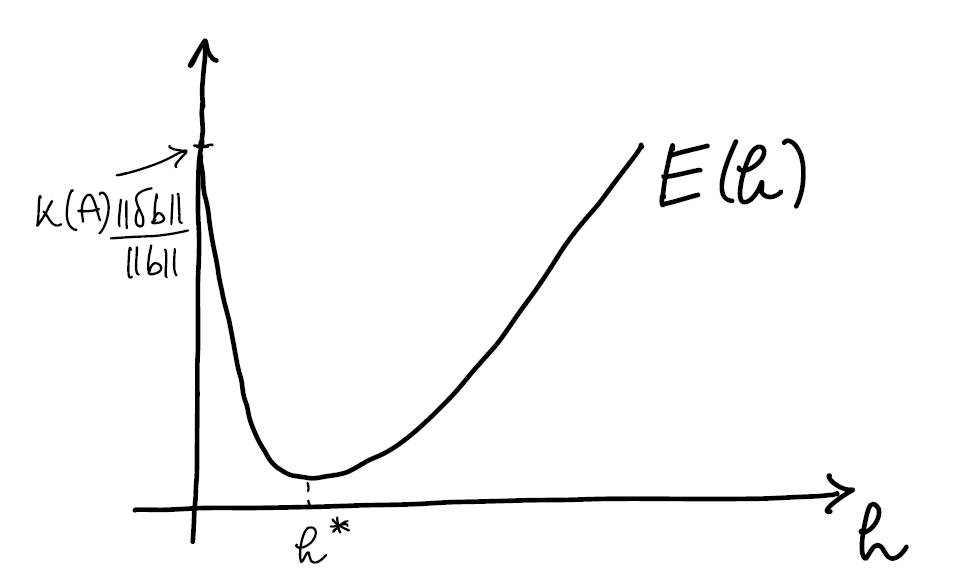
\includegraphics[scale=0.5]{lez20_pag35.png}    
\end{center}
Si noti l'analogia col caso della derivazione numerica: anche qui conviene stimare $h^*$ (stima che è molto più difficile che nel caso della derivazione numerica e per cui si usano spesso tecniche statistiche o euristiche) prendendo un parametro vicino a quello ottimale in modo che minimizzare l'errore (perdendo comunque precisione rispetto all'errore sui dati perchè si "eredita" l'instabilità del problema ma calcolando una soluzione che può spesso essere accettabile in pratica).
\end{document}